\documentclass[a4paper, 11pt]{article}
\usepackage{amsmath}
\usepackage{amssymb}
\usepackage[T1]{fontenc}
\usepackage[utf8x]{inputenc}
\usepackage{lmodern}
\usepackage{graphicx}
\graphicspath{ {./images/} }
\usepackage[english]{babel} 
\usepackage{natbib}
\usepackage{cite}
\usepackage[parfill]{parskip}
\usepackage{enumerate}
\usepackage{float}%for image positions
\usepackage{hyperref}
\hypersetup{
  colorlinks,
  citecolor=black,
  filecolor=black,
  linkcolor=black,
  urlcolor=black
}
\usepackage{amsthm}
\newtheorem{theorem}{Theorem}[section]
\newtheorem{lemma}[theorem]{Lemma}
\newtheorem{proposition}[theorem]{Proposition}
\newtheorem{axiom}[theorem]{Axiom}
\newtheorem{invariant}[theorem]{Invariant}
\newtheorem{breakpoint}[theorem]{Breakpoint}
\newtheorem{problem}{Problem}
\newtheorem{definition}{Definition} 
\usepackage{algorithm}
\usepackage{algpseudocode}
\usepackage{pifont}
\usepackage{multirow,array}
\usepackage{centernot}
\usepackage{listings}
\usepackage{xcolor}
\usepackage{color}

\lstdefinestyle{base}{
  language=C,
  emptylines=1,
  breaklines=true,
  basicstyle=\ttfamily\color{black},
  moredelim=**[is][\color{red}]{@}{@},
}

\lstdefinestyle{java}{
  language=Java,
  showspaces=false,
  showtabs=false,
  breaklines=true,
  showstringspaces=false,
  breakatwhitespace=true,
  commentstyle=\color{green},
  keywordstyle=\color{blue},
  stringstyle=\color{red},
  basicstyle=\ttfamily,
  moredelim=[il][\textcolor{grey}]{$$},
  moredelim=[is][\textcolor{grey}]{\%\%}{\%\%},
}


\usepackage{comment} % enables the use of multi-line comments (\ifx \fi) 
\usepackage{lipsum} %This package just generates Lorem Ipsum filler text. 
\usepackage{fullpage} % changes the margin

\begin{document}
\noindent
\large\textbf{Homework 2} \hfill \textbf{Kim Hammar} \\
\normalsize ID2208 \hfill  \textbf{Mallu} \\
Programming Web-Services \hfill Due Date: 7 February 2017\\

\section*{Problem Statement}
This report covers the work done in an assignment on programming WebServices. The given task was to implement flight-ticket reservation services as web services. Further more both the top-down and bottom-up approaches to developing web services should be practiced.
\section*{Main problems and solutions}
\begin{itemize}
\item \textit{Bottom-up approach} - This task included using JAX-WS library \citep{jax_ws} in java to implement webservices by first developing java classes and interfaces and then using \texttt{wsgen} tool to generate WSDL and XML Schema files.
\item \textit{Top-down approach} - Opposite development chain compared to bottom-up. Start by developing WSDL and XML schema files and then use the \texttt{wsimport} tool to generate Java classes and interfaces.  
\end{itemize}

\subsection*{Bottom-up}
JAX-WS uses annotations to declare service endpoints and interfaces. It is supringisngly little difference between implementing a webservice and a regular java program since the annotations are mainly in one file which defines the API for your webserivce. The business-logic for the service is implemented like a regular java-program except one important part: JAXB-annotations. JAX-WS uses JAXB under the hood for marshalling and unmarshalling, this means that you can return java-objects from your webmethods and not just simple-types like strings and integers. To be able to do this you need to annotate classes that your webmethods returns in order for JAXB to  know how to marshall and unmarshall the objects. For example a PriceEntry object sent over the wire as a result of the GetPriceList webmethod can be annotated as follows:
\begin{lstlisting}[frame=single,style=java]
@XmlRootElement(name="PriceEntry")
public class PriceEntry {
    @XmlElement(name = "Itinerary")
    private Itinerary itinerary;
    @XmlElement(name = "Price")
    private float price;
  \end{lstlisting}

\subsection*{Top-down}
We have implemented booking and issuing of tickets services as top down web services, for top down web service the first step is to generate a wsdl file first which completely describes the web service to be implemented, and then we generate java from this wsdl file using \texttt{wsimport} command. For this task, we have created \texttt{FlightReservationServiceTopDown.wsdl} as core step and then generated further java files. This task also included defining the XML types in XML schema. We found that designing a WSDL file was very simple and efficient way to build java-webservices however we encountered some special effects we did'nt know in advance which is presented in the following section.

\subsubsection*{Our experience from automatic generation with wsgen and wsimport}
The whole idea of top-down vs bottom-up approach to webservices development exists because there is a good match between XML structures and in particular object-oriented languages like java. Access to tools like \texttt{wsgen} and \texttt{wsimport} means that it is possible to automate generation of java-files from WSDL/XML and vice-versa.

In this assignment we applied both directions and it works well but we discovered that the generation highly depends on what structure you use in your wsdl-file and your java-file. For instance how you define your types in XML schema, using anonymous complex-types inside element definitions results in java files looking something like this:
\begin{lstlisting}[frame=single,style=java]
  public class ItineraryType {
        @XmlElement(
        name = "Flights"
    )
    protected List<ItineraryType.Flights> flights;

    public static class Flights {}
  }    
\end{lstlisting}
In essence the generation tool creates static inner classes for local elements in XML Schemas and stand-alone java classes for global elements. This ofcourse is not a problem, and it will result in the same SOAP-messages on the wire, 
but it had the consequence that we could'nt use the same client for the bottom-up implementation as the top-down implementation as for example the generated \texttt{ItineraryType.Flight} in the top-down implementation cannot be interchanged with the \texttt{Flight} class used in bottom-up implementation and thus the java-client needs to know which class to parse into. 


\subsection*{Implementation}
Both the bottom-up and top-down implementation results in the same result, a webservice that uses JAX-WS library and Document-style SOAP communication over the default SOAP-HTTP binding.
\begin{figure}[H]
  \begin{center}
    \scalebox{0.7}{
      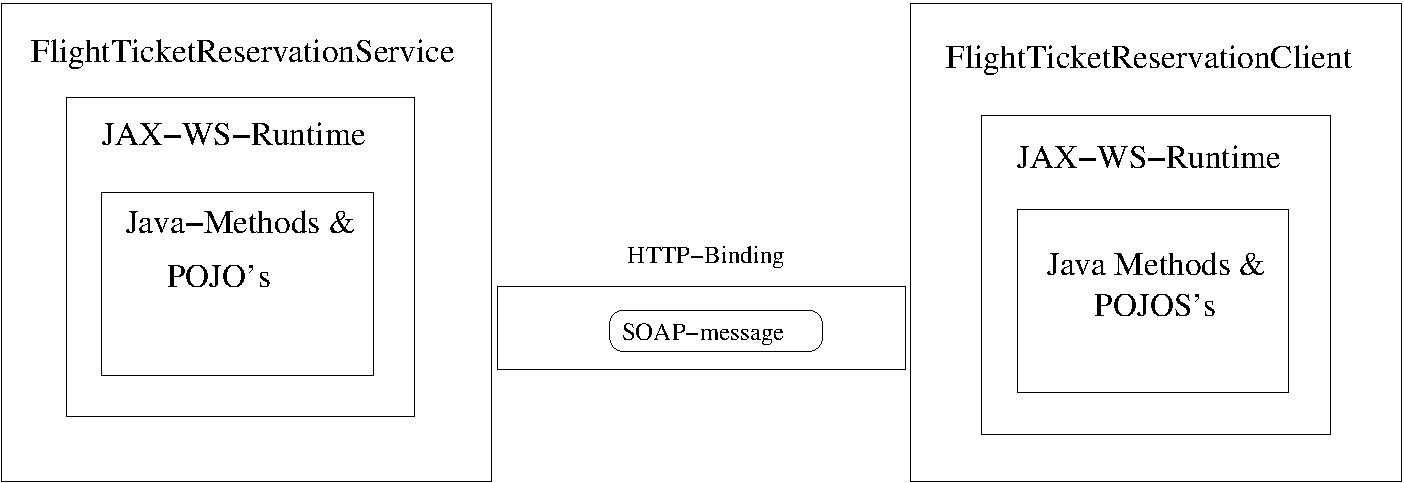
\includegraphics{fig.pdf}
    }
    \caption{WebService Implementation with JAX-WS}
    \label{fig:fig}
  \end{center}
\end{figure}

\subsection*{SOAP}
Using headers to add functionality to SOAP messages is known as vertical extension \citep{coursebook}. Perhaps the most canonical case to use SOAP headers to extend messages and protocols is to add security, since this is a typical requirement that might not be required at first deployment but as the service matures it might become a necessity. In our implementation of the flight-ticket reservation service we use a very ad-hoc authentication/authorization solution. First of all, credentials are sent in plaintext, and second, the security token is sent as an \textit{argument} to each invocation which clutters the interface and gives poor separation of concerns.
\begin{lstlisting}[frame=single,style=base]
<S:Envelope xmlns:S="http://schemas.xmlsoap.org/soap/envelope/">
    <S:Body>
        <ns2:getItineraries xmlns:ns2="http://flight_reservation">
            <arg0>Stockholm</arg0>
            <arg1>Mumbai</arg1>
            <arg2>@ID2208_AUTH_TOKEN@</arg2>
        </ns2:getItineraries>
    </S:Body>
</S:Envelope>
\end{lstlisting}
A better idea would be to employ a security solution utilizing SOAP intermediaries and WS-Security, however that is out of scope of this tutorial, but atleast we can achieve a better service-design by sending the security-token as part of the SOAP header instead of sending it as an invocation-argument.
\begin{lstlisting}[frame=single,style=base]
<S:Envelope xmlns:S="http://schemas.xmlsoap.org/soap/envelope/">
    <S:Header>
        <ns2:Token>@ID2208_AUTH_TOKEN@</ns2:Token>
    </S:Header
    <S:Body>
        <ns2:getItineraries xmlns:ns2="http://flight_reservation">
            <arg0>Stockholm</arg0>
            <arg1>Mumbai</arg1>
        </ns2:getItineraries>
    </S:Body>
</S:Envelope>
\end{lstlisting}
There are many advantages with this approach:
\begin{itemize}
\item Separating the authentication from the method invocation means that we can later improve the security solution and change the API without having to change the interface of every operation.
\item Having the authentication information in the header means that we could develop a solution where SOAP intermediaries handles the authentication and the application don't have to be aware of it.
\end{itemize}
\section*{Conclusions}
JAX-WS library allows you to develop web services in java without having to do much manual work with XML. However, to achieve good design for a web service you still need a satisfactory understanding of the underlying technologies and formats. Two main approaches to developing web services nowadays when using java are top-down and bottom-up, which one to prefer depends on the situation. In general it requires more knowledge to do the top-down approach but it can also be more powerful.

\section*{Attachments}
Documented source code, WSDL files, XML Schemas and SOAP-message dumps can be found in the attached zipfile. See README.MD in the root directory for instructions how to execute and build the program.

\bibliography{references}{}
\bibliographystyle{plain}
\end{document}